%%%%%%%%%%%%%%%%%%%%%%%%%%%%%%%%%%%%%%%%%%%%%%
%%%%% Default format: 12pt single column %%%%%
%% 12pt is the minimum font size allowed !! %%
%% This applies to everything, including    %%
%% references, figure captions, and tables  %%
%% ==> Proposals not compliant to this will %%
%%     be rejected. See Section 5.3.1 in    %%
%%     the ALMA Proposer's Guide            %%
%%%%%%%%%%%%%%%%%%%%%%%%%%%%%%%%%%%%%%%%%%%%%%

\documentclass[12pt,a4paper]{article}  %% DO NOT CHANGE to 11pt or less !

\usepackage[numbers]{natbib}
\usepackage{hyperref}
\usepackage{graphics,graphicx}
\usepackage{xspace}
\usepackage{amsmath,amssymb}
\newcommand{\msun}{\ensuremath{\mathrm{M}_\odot}\xspace}
\newcommand{\kms}{\ensuremath{\mathrm{km~s}^{-1}}\xspace}
\newcommand{\percc}{\ensuremath{\mathrm{cm}^{-3}}\xspace}
\newcommand{\persc}{\ensuremath{\mathrm{cm}^{-2}}\xspace}

\newcommand{\mnras}{MNRAS}

\usepackage[table]{xcolor}% http://ctan.org/pkg/xcolor


\usepackage{titlesec}
\titlespacing{\section}{12pt}{6pt}{8pt}
\titlespacing{\subsection}{12pt}{6pt}{8pt}

\newlength\tindent
\setlength{\tindent}{\parindent}
%\setlength{\parindent}{0pt}
\renewcommand{\indent}{\hspace*{\tindent}}


\usepackage{tcolorbox}
\usepackage{paralist}

\renewenvironment{thebibliography}[1]{%
  %\section*{\refname}%
  \textsc{\textbf{References:}}
  \let\par\relax\let\newblock\relax%
  \inparaitem[{[}1{]}]}{\endinparaitem}
  
\usepackage{etoolbox}
\makeatletter
\patchcmd{\@lbibitem}{\item[\hfil\NAT@anchor{#2}{\NAT@num}]}{\item[\NAT@anchor{#2}{\NAT@num}]}{}{}
\makeatother



%%%%%%%%%%%%%%%%%%%%%%%%%%%%
%%%%%% Page dimensions %%%%%
%%%%%%  DO NOT CHANGE  %%%%%
%%%%%%%%%%%%%%%%%%%%%%%%%%%%

\textheight=247mm
\textwidth=180mm
\topmargin=-7mm
\oddsidemargin=-10mm
\evensidemargin=-10mm
\parindent 10pt

%%%%%%%%%%%%%%%%%%%%%%%%%%%%%
%%%%% Start of document %%%%% 
%%%%%%%%%%%%%%%%%%%%%%%%%%%%%

\begin{document}
\pagestyle{plain}
\pagenumbering{arabic}
\newcommand{\arcsec}{"}


 
% The title, abstract and list of investigators should NOT be included in the
% Scientific justification. The title and abstract are put automatically on the cover page.

%%%%%%%%%%%%%%%%%%%%%%%%%%%%%%%%%%%%%%%%%
%%%%% Body of science justification %%%%%
%%%%%%%%%%%%%%%%%%%%%%%%%%%%%%%%%%%%%%%%%

%% ENTER TEXT, FIGURES AND TABLES BELOW
%% Minimum font size for all text, references, figure captions, and tables is 12pt
%% Proposals not compliant to this will be rejected. See Section 5.3.1 in the ALMA Proposer's Guide.


\vspace{-0.5em}
\begin{center}
\large
\textbf{{Scientific Justification: \emph{The MUBLO is a unique source}}}
\end{center} 
\vspace{-0.5em}


% ALMA uses two systems to review the proposals submitted in the Main Call.
% All proposals requesting less than 50 h on the 12-m Array and all ACA stand-alone proposals
% requesting less than 150 h on the 7-m Array will be reviewed by Distributed peer review
% (see Sections 5.7.1 and 1.2.2 of the Proposer's Guide).
% All Large Programs will be reviewed by Panels. 
% Additionally, both systems will follow a dual-anonymous procedure, in which the proposers
% do not know who are the reviewers and the reviews do not who are the proposers.
%
% Please refer to the guidelines before writing your proposal:
%     https://almascience.org/proposing/alma-proposal-review/dual-anonymous
%
% In the following part, describe the scientific background of the project,
% pertinent references and previous work relevant to this 
% proposal, together with any figures and tables that you judge necessary
% (use the following two examples as templates, or remove)
% Please do not disclose the name(s) of the proposer(s), and write the proposal in a way
% such that the proposer(s) cannot be identified. 
 
%-----------------------------Figure Start---------------------------

% The 'scale' parameter below allows you to scale the figure so that it fits within the page.
% In this case the figure was scaled to 20% of its original size.
% Note: for .png files one has to use pdflatex, not classic latex
%
% Minimum font size for references: 12pt 
% Proposals not compliant to this will be rejected. See Section 5.3.1 in the ALMA Proposer's Guide.
A compact (barely resolved at 1\arcsec~ resolution) millimeter source with extremely broad line width has recently been detected in the Galactic Center \citep{Ginsburg2024}.
This source, G0.02467-0.0727, called the Millimeter Ultra-Broadline Object (MUBLO) by those authors, is detected both in continuum and in very broad line emission (FWHM $\sim165~\kms$; Fig. \ref{fig:coarse_spectra}) in emission lines of CS and SO.
It is not detected at any other wavelength from X-ray to radio.
Many hypotheses for the nature of this source have been evaluated, and it was found that none are presently satisfactory (see Table \ref{tab:hypotheses}).
The MUBLO is an exciting mystery that, at least for now, can only be further investigated by ALMA.

\begin{tcolorbox}
\noindent 
We propose observations to test the two most promising possibilities: that the MUBLO is a disk around an intermediate-mass black hole, or that it is the remnant of a stellar merger.
\end{tcolorbox}

\begin{figure}[htp!]
    \centering
    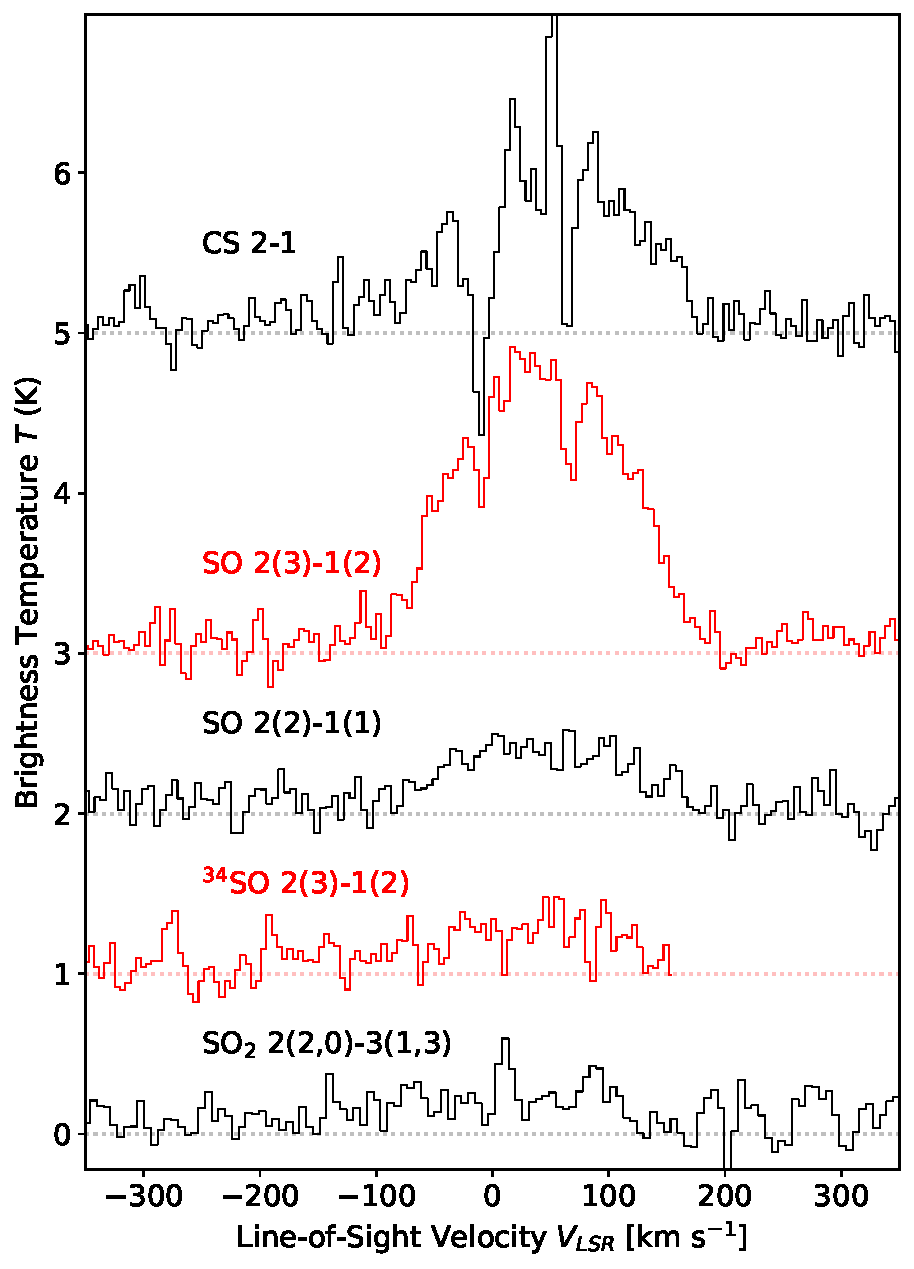
\includegraphics[width=0.36\textwidth]{figures/CSandSO_Overlays.pdf}
    %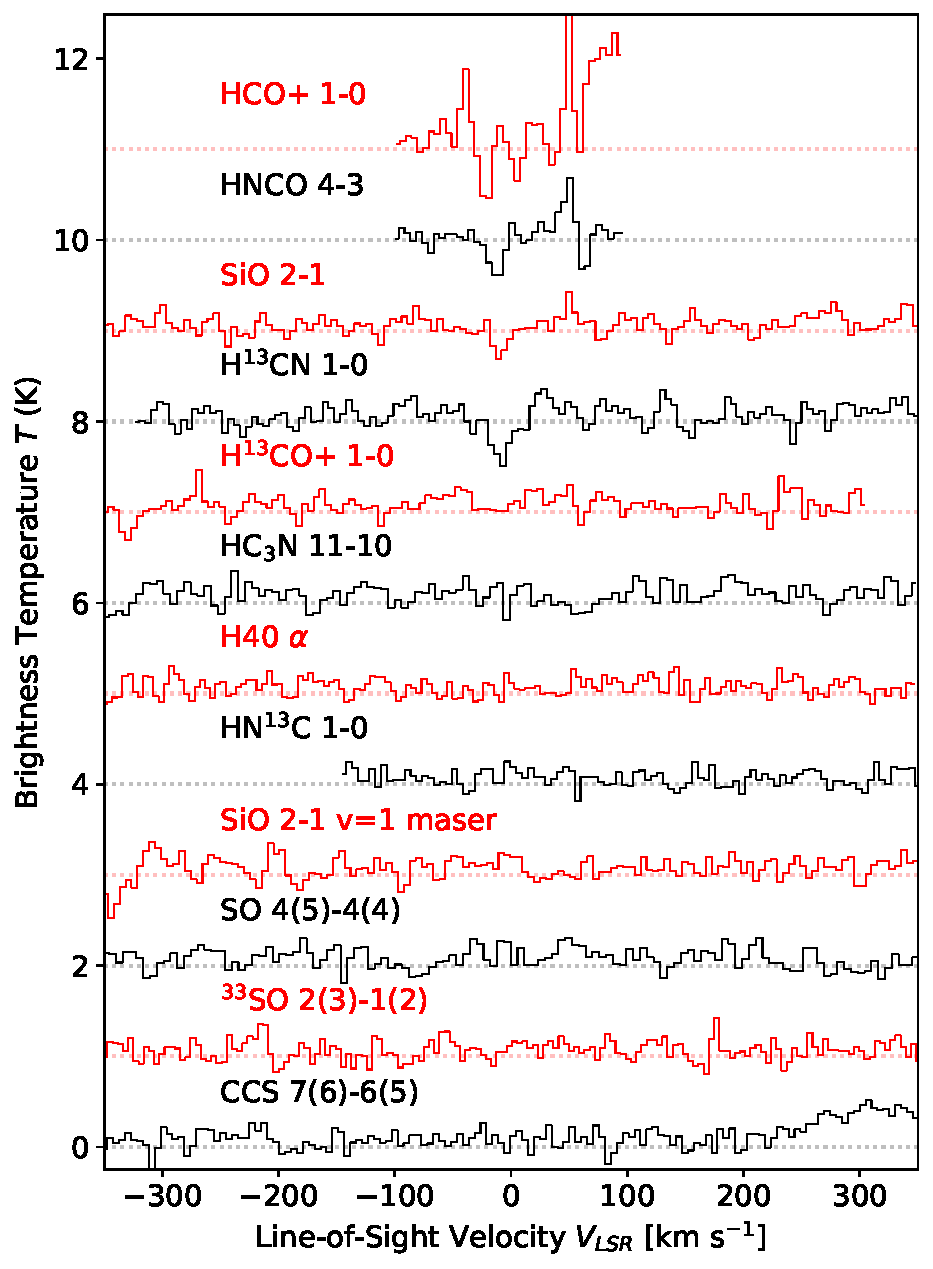
\includegraphics[width=0.49\textwidth]{figures/NonDetection_Overlays.pdf}
    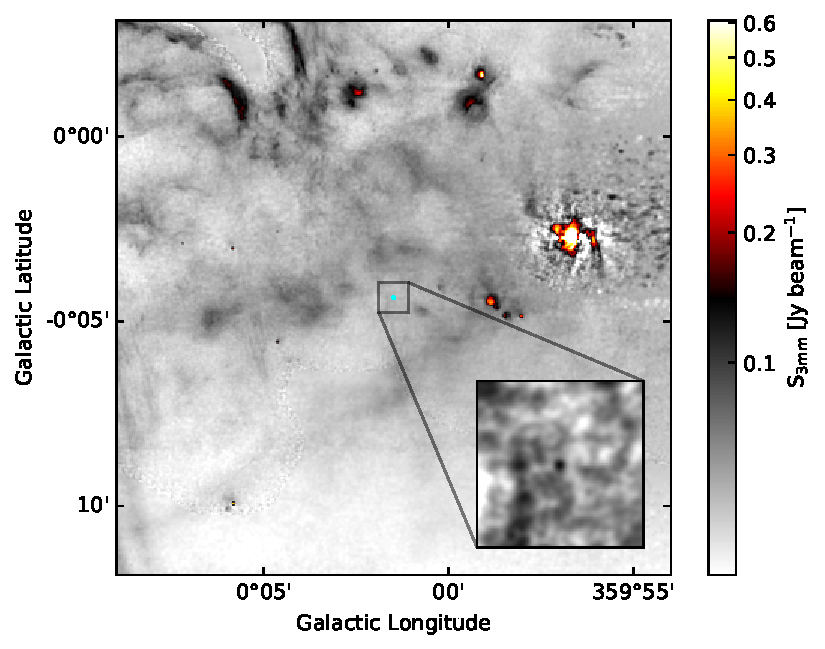
\includegraphics[width=0.63\textwidth]{figures/MUSTANG3mmContext.pdf}
    \caption{(left) Spectra of detected lines in ALMA archival spectral coverage.
    Only CS, SO, and SO$_2$ are detected. (right) Continuum image showing the MUBLO in spatial context. Sgr A* is on the right side of the zoomed-out image.
    %Figure \ref{fig:coarse_spectra_withTP} shows the same data with the Total Power spectra, which covers larger physical scales ($\sim2$ pc), overlaid.
    }
    \label{fig:coarse_spectra}
\end{figure}

\textbf{Source property summary:}
The continuum emission has a spectral index $\alpha\approx3.3$, suggesting that it is from dust.
It is detected in all three ALMA observations that overlap on the sky (two 12M data sets in B3, one 7M in B7) and an SMA DDT observation in B6 (priv. comm.).
The line emission is detected in several transitions of CS and SO isotopologues and exhibits a line width FWHM $\approx165$ \kms (Fig. \ref{fig:coarse_spectra}).  The line profile appears Gaussian.
The emission is weakly spatially resolved in existing 2" resolution data, coming from an area on the sky $\lesssim1"$ in diameter \mbox{($\lesssim10^4$ AU at the distance of the GC).}
The centroid velocity is $v_{LSR}\approx40-50$ \kms, which suggests the object is genuinely in the Galactic Center and is possibly associated with the 50 \kms cloud.
There is a tentative detection (10$\sigma$ accounting for statistical error only; the systematic errors are difficult to quantify) of a velocity gradient of 11000 \kms pc$^{-1}$.
Two independent SO lines are detected, and assuming LTE conditions, the gas temperature is $T_{rot}\approx 14$ K, much colder than seen in typical Galactic Center clouds (Fig. \ref{fig:LTErotationdiagram}).
However, with the limited set of lines presently detected, it is also possible that the emission is coming from low-density, subthermally excited gas.
Despite the high velocity dispersion, no emission is observed from SiO in the observed SiO $J$\;=\;2-1 transition, suggesting that there are no strong ($\gtrsim10~\kms$) shocks in the molecular gas.
There are no detections at other wavelengths, including X-ray with Chandra, XMM-Newton, and NUSTAR, infrared with HST and Spitzer, and radio with VLA and MEERKAT.
ALMA is the only telescope capable of performing followup observations.


\textbf{What is it?}
There are several possible explanations for this source that have been evaluated, including protostellar outflow, explosive outflow, collapsing cloud, evolved star, stellar collision, high-velocity cloud, intermediate mass black hole, and background galaxy (Table \ref{tab:hypotheses})\citep{Ginsburg2024}.
Most of these conceptual models are inconsistent with the data in at least one way, but the data are not presently very constraining.
In this proposal, we will image the source in the continuum at high resolution to verify the dusty nature of the source and map its internal structure.
With the higher resolution observations of the previously detected lines, we will determine how concentrated the line emission is.  
If line emission is detected, we will test whether the velocity gradient is real and resolve the kinematic structure to determine whether it's an outflow, a disk, or something else entirely.


\begin{table}[htp]
    \centering
    \begin{tabular}{|c|c|c|c|c|c|c|c|}
         \hline
         Hypothesis & Broad & No IR & No X-ray & Gaussian & $X_{SO}$, $X_{CS}$ & No SiO & Size \\
         \hline
         IMBH \cellcolor{yellow!25} & \cellcolor{green!25}+ & \cellcolor{green!25}+ & \cellcolor{red!25}- & \cellcolor{red!25}- & & & \cellcolor{green!25}+\\
         \hline
         Stellar Merger \cellcolor{yellow!25} & \cellcolor{green!25}+ & \cellcolor{red!25}- & & & \cellcolor{green!25}+ & \cellcolor{red!25}-  & \cellcolor{green!25}+\\
         \hline
         YSO  \cellcolor{yellow!25} & \cellcolor{red!25}- &  \cellcolor{green!25}+ & & \cellcolor{green!25}+ & \cellcolor{red!25}- & \cellcolor{red!25}- &\cellcolor{green!25}+  \\
         \hline
         Protostellar Outflow \cellcolor{orange!25} & \cellcolor{green!25}+ & \cellcolor{red!25}- & & \cellcolor{red!25}- & \cellcolor{red!25}- & \cellcolor{red!25}-  & \cellcolor{red!25}-\\
         \hline
         Supernova \cellcolor{orange!25}& \cellcolor{green!25}+ & \cellcolor{green!25}+ & \cellcolor{red!25}- & & \cellcolor{red!25}- & \cellcolor{red!25}- & \\
         \hline
         (pre)Planetary Nebula \cellcolor{orange!25}& \cellcolor{red!25}- & \cellcolor{red!25}- & &  \cellcolor{green!25}+ & \cellcolor{green!25}+ & \cellcolor{red!25}- & \\
         \hline
         Background Galaxy \cellcolor{red!25}& \cellcolor{green!25}+ & \cellcolor{red!25}- & & & \cellcolor{red!25}- &  & \cellcolor{red!25}-\\
         \hline
         High-velocity Compact Cloud  \cellcolor{red!25}& \cellcolor{green!25}+ & \cellcolor{green!25}+ & \cellcolor{green!25}+ & \cellcolor{red!25}- & \cellcolor{red!25}- & \cellcolor{red!25}- & \cellcolor{red!25}-\\
         \hline
    \end{tabular}
    \caption{Hypotheses that have been evaluated and the evidence for (green +) and against (red -) them; blank means the evidence is neither for nor against.
    The overall weight given to the hypothesis is given by its color code - yellow are not entirely ruled out, orange are strongly disfavored but still possible, and red are very low likelihood.
    There is at least one strong item of evidence against each hypothesis considered.
    }
    \label{tab:hypotheses}
\end{table}


The most exciting possibilities for this source are that it is an intermediate mass black hole (IMBH) or  a stellar merger remnant.
In these cases, we expect to see compact structures at $\sim100-500$ au resolution - for an IMBH, from the Keplerian outer disk; from a merger remnant, we expect to see a messier, multi-directional explosion or an expanding ring.
For an IMBH, we might expect to see only a simple, isolated, Keplerian disk heated only by viscous processes,
while for a stellar merger remnant, an outflow shaped only by the merger event is likely (Figure \ref{fig:whatwecouldsee}, right, shows what this might look like based on merger remnant CK Vul).
There are other, somewhat more mundane but still exciting possibilities, like an isolated high-mass YSO.
For a YSO, we expect to see connections to the surrounding environment or parental core, 
For an accreting YSO, there should be a strong central heating source.

Observations at the high proposed physical resolution ($70$, $130$ and $500$ AU proposed in B9, B7, and B3, respectively) will be able to definitively test the IMBH model, since it predicts extreme kinematics on very small scales.
In such a model, the line emission is coming from much smaller scales and therefore has a high enough surface brightness to be detected despite our modest proposed brightness sensitivity.
The archival data have 2" (16,000 AU) resolution, and a 2000 AU offset was measured between the red- and blue-shifted lobes of the object by centroiding, so we expect to be able to measure down to at least $\sim20$ AU with the proposed higher-resolution and higher-sensitivity data.
An orbit of $v=165$ \kms at $r=20$ AU requires a central object with $M\sim600$ \msun, so we will resolve the disk kinematically for any more massive object.
Distinguishing the other possibilities (YSO vs merger remnant) will come down to details of the substructure and connections to the environment; YSOs should have many neighbors, while mergers of main-sequence or evolved stars are likely to be entirely isolated.





\vspace{-0.5em}
\begin{center}
\large
\textbf{{Observations \& Analysis Plan: \emph{Resolve the source, measure its SED}}}
\end{center} 
%\vspace{-0.5em}
\begin{tcolorbox}
\noindent 
We will observe the target in B3, B7, and B9 with 0.065", 0.016", and 0.009" resolution, respectively, to resolve the source structure, confirm its dusty nature, and map its temperature.
\end{tcolorbox}


Our main science objective is to resolve the source and map its continuum structure.
All of the proposed models can be readily distinguished by observations with 70 au (0.009") and 130 au (0.016") resolution, which is what we request in B9 \& B7.
At 500 au resolution (0.065"), the maximum achievable in B3, in conjunction with the B7 and B9 data, we will measure a resolved spectral index to test the origin of the continuum emission.
By observing all three bands with commonly-detected angular scales (we request 1" LAS recovery in all bands), we will map out the resolved temperature structure in the dust; Fig. \ref{fig:LTErotationdiagram} shows that the dust is cold enough that the B9 data strongly differentiate different temperature models.

By resolving the continuum source, we can determine whether it is circularly symmetric (which would favor overall spherical symmetry) or flattened (favoring a disk).
However, these two possibilities are far from a complete list - with the proposed high-resolution observations that resolve the structure of the continuum, we can simply see what is there.


%(2) Measure the gas excitation.  Is the molecular gas \emph{really} only 13 K?  


%(3) What other lines does the MUBLO emit?

%While our observations will cover a wide range of species, we focus on the CS and SO molecules, since they are both clearly detected in existing B3 data.

% Please describe the observations to be made and their specific
% purpose, with a clear explanation of the need for, and 
% appropriateness of, ALMA Cycle 10 data.  

%No matter the nature of this source, it is clear that we need to follow it up.  The key observations to distinguish the above possibilities are:

% \begin{enumerate}
%     \item Resolved observations of the structure of the molecular feature.  We should aim for resolution $10\times$ better than currently achieved, which is straightforward with ALMA and can be requested at several wavelengths in the upcoming Configuration 6 in June 2024.  This is the key measurement, since the shape of the kinematic structure should be different for all of the above hypotheses (e.g., a circumstellar disk will have a Keplerian curve, while a galactic inner disk would likely be either solid-body or flat).  
%     \item A better molecular inventory.  Observations of HCN, HCO+, HNCO would be nice.  CO isotopologues, including very rare ones (C$^{17}$O, $^{13}$C$^{18}$O) should be included to avoid CMZ optical depth problems.  We should brainstorm other important species.  For example, H$_2$CS and H$_2$CO may be useful for better constraining the sulfur chemistry and the gas temperature.
%     \item A better physical characterization.  Additional transitions of CS and SO are necessary to measure the excitation.  Is the temperature really as low as we measure, or is the density low and we are instead seeing non-LTE conditions?
% \end{enumerate}

\begin{figure}[htp]
    \centering
    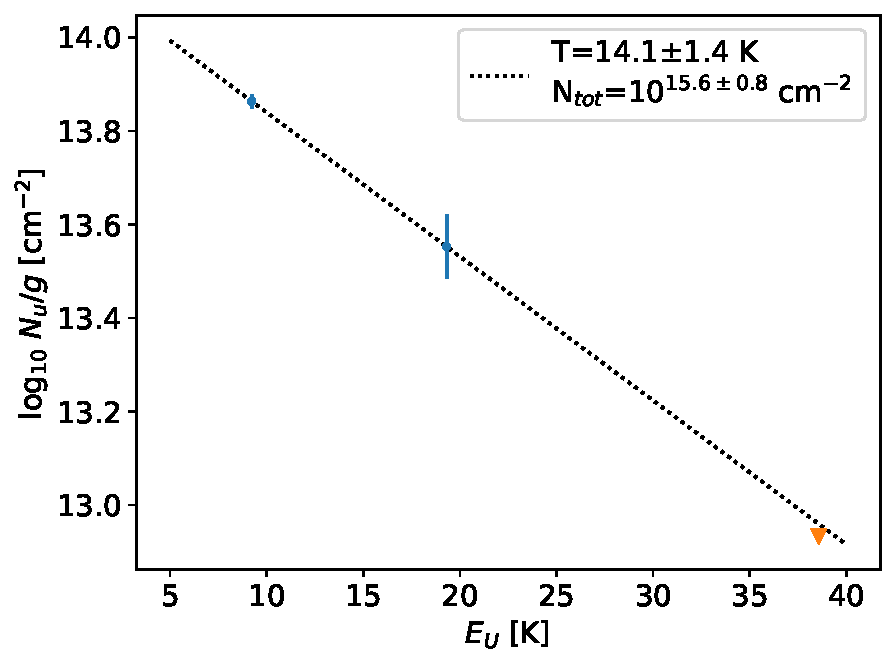
\includegraphics[width=0.49\textwidth]{figures/LTE_rotationdiagram_fit.pdf}
    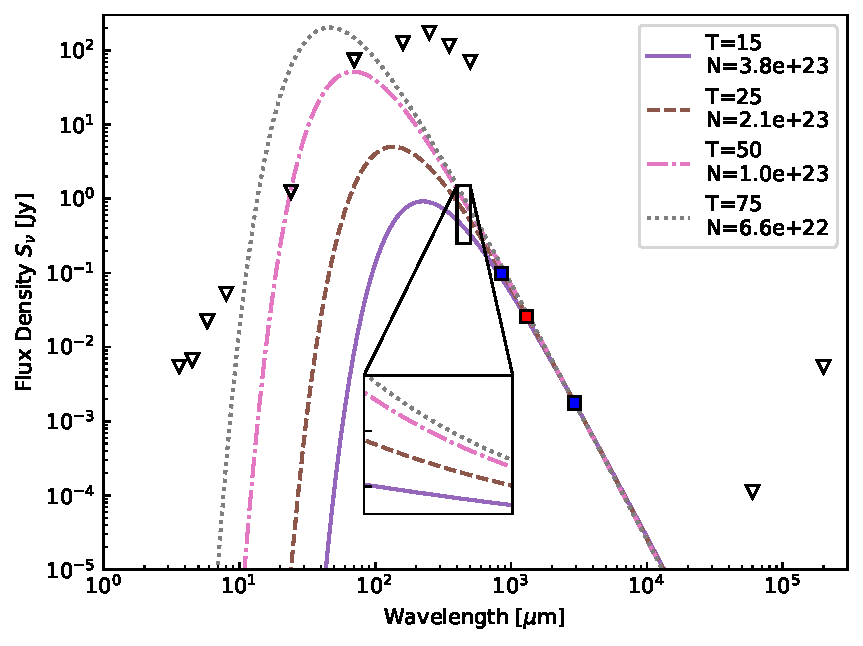
\includegraphics[width=0.49\textwidth]{figures/SED_with_planned_B9.pdf}
    \caption{(left) Rotation diagram showing the best fit for the SO lines.
    With only two lines, we cannot tell whether the lines are in LTE and genuinely cold or are instead sub-thermally excited.
    (right) Continuum spectral energy distribution. Except for the ALMA (850 $\mu$m and 3mm; blue) and SMA (1.3mm; red) data points, all are upper limits.  The modified blackbody curves show that the dust temperature is limited to be $T_D<50$ K.
    The inset shows where the B9 measurement will be made, with the Y-axis on a linear scale, demonstrating that this SED data point will efficiently measure the dust temperature anywhere it is below $T<50$ K.
    }
    \label{fig:LTErotationdiagram}
\end{figure}

\textit{Technical Justification:}
Our sensitivity goal is to detect the continuum if it is nearly uniformly spread across the object, which is the worst-case scenario.
At B3, that is a $\sim100\times$ dilution, requiring $\approx 0.02$ mJy sensitivity, which is achievable in 3.5h.
At B7, the source is many times brighter, but the original detection was with the 7m array and had $\approx 4"$ resolution, so we request comparable sensitivity $\approx0.025$ mJy, requiring 4h.
For both of these previously-observed bands, we aim to recover a largest angular scale of 1", which is the deconvolved source size reported in \citep{Ginsburg2024}; this requires a second 12m array configuration with relatively short total time.
We request a B9 observation with 0.009" resolution and 0.25 mJy sensitivity to make the highest-resolution possible image.
In order to achieve a largest angular scale of 1" while resolving 0.065" scales for comparison to B3 and B7 and perform temperature measurements, we request a second B9 science goal with two configurations.
The low-resolution SED shown in Figure \ref{fig:LTErotationdiagram} shows that a 460$\mu$m data point is highly sensitive to the dust temperature.
The B9 observations require 3.5h across all three configurations.
The total request is roughly 11h.
%For all three bands, we also request shorter-baseline configurations to enable cross-comparison between the data sets and to ensure that, between archival data and the new proposed observations, no angular scales are missed.

The requested line sensitivity is about 46 K at B3, 5 K at B7, and 14 K at B9, all in 1 \kms channels at 0.065" resolution.
At this sensitivity, we only expect to detect line emission in B7 unless there are compact, high-brightness regions.
Such concentration of the emission into compact regions is possible, but upper limits on the compactness of the SO and CS emission will provide strong constraints on the source of the emission.
This sensitivity improves to 5.5 K, 0.6 K, and 1.7 K in each band when averaged over 70 \kms, just under the HWHM, which is the minimum spectral resolution needed to resolve a velocity gradient.
If line emission is detected, it will be used to measure the gas kinematics, distinguishing between outflow, disk, or other motion.
\vspace{0.2em}



% a 5 mJy signal in an 0.2" beam and a 5 \kms channel width at 5$\sigma$.
% We adopt 5 \kms as our sensitivity target because, although the line is very broad, we need to detect it in many channels to measure the line shape, and we need to remove line-of-sight clouds from the profile before fitting.
% This is a similar brightness sensitivity to the archival observations, but in a smaller beam so that we can confirm (or reject) the velocity gradient measurement.
% The peak line intensity observed in B3 in the two brightest lines is 30 mJy in SO 3(2)-2(1) and 18 mJy in CS 2-1.

%We target Band 3 and 7 to measure the dust spectral index and additional lines of both CS and SO at high resolution.
%While we have a continuum detection in Band 7 with the ACA, it is at poor 4" resolution and does not resolve the continuum source or detect line emission.
%The B7 data will achieve high signal-to-noise in the continuum with expected noise $\sigma_{350 GHz}=0.03$ mJy/beam yielding S/N $> 2000$ if the source remains unresolved.
%The B4 data will have $\sigma_{140 GHz}\approx5$ $\mu$Jy, yielding predicted S/N$\sim1000$.
%With this high signal-to-noise, we anticipate self-calibration will be needed to maximize the continuum sensitivity.


% We performed basic RADEX modeling adopting the LTE-inferred column density N(SO) = $4\times10^{15}$ \persc and $T=13$ K.
% The Band 4 SO 3(4)-2(3) line is the key diagnostics: 3(4)-2(3) will be detectable at $T_B>2.5$ K ($>5\sigma$) for T=13 K, $n\geq5\times10^4$ \percc, so we can use it to constrain the gas density.
% There are several other SO lines in both bands that the RADEX model predicts will not be detected, but they come along for free.

%The CS 3-2 and 7-6 provide an independent measurement of the rotational temperature and density conditions.
%For T=13 K, CS 3-2 will be detected at $>5\sigma$ for $n\geq5\times10^5$ \percc; it should be detected for any plausible combination of physical parameters.
%By contrast, the CS 7-6 line will only be detected if the density and temperature are both high ($n>10^6$ \percc, $T>50$ K), so it is an excellent diagnostic of high-excitation conditions.
%The model predicts the SO 8(8)-7(7) line will be 0.1 K (0.4 mJy) if SO is in LTE at 13 K, which is below our practical detection limit. 
% 
%and it would remain detectable down to $n(H_2)>5\times10^5$ \percc at the assumed temperature $T=13~K$.

\begin{figure}
    \centering
    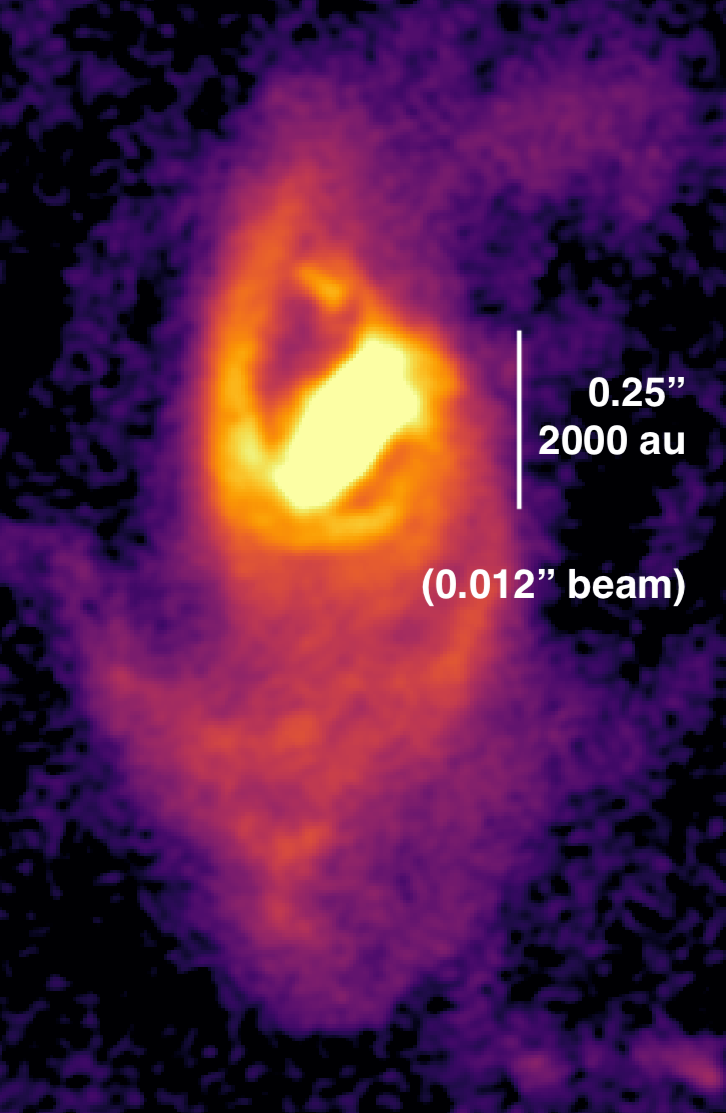
\includegraphics[width=0.30\textwidth]{figures/proposal_figures/sgrc_disk_zoom_scalebar.png}
    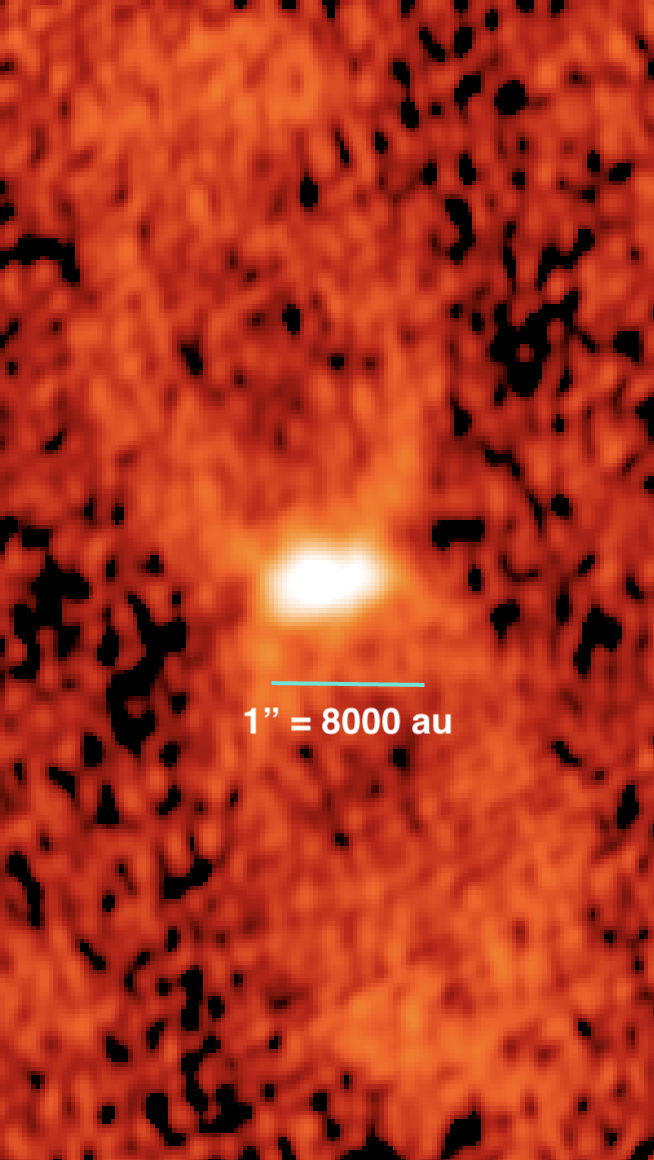
\includegraphics[width=0.26\textwidth]{figures/proposal_figures/CKVulcontinuum.png}
    \caption{Example images of what we might detect in the proposed observations.
    Left shows a large ($\sim2000$ au), massive (5 \msun) disk around a YSO \citep{Lu2022} observed in the Galactic Center cloud Sgr C with ALMA at B7 in C10 in 2023.
    Right shows the merger remnant CK Vulpecula \citep{Eyres2018} observed with ALMA in B6 scaled to the distance of the Galactic Center. 
    This remnant of a white dwarf-brown dwarf merger bears a different kind of disk and shows no connection to the broader environment.
    The central source in each of these objects has a similar continuum flux (to within a factor of a few) to the MUBLO in the 2" beam that is presently the only detection of the MUBLO.
    }
    \label{fig:whatwecouldsee}
\end{figure}
% CK Vul image member.uid___A001_X129e_X258.CK_Vul_sci.spw25_27_29_31.cont.I.pbcor.fits

%\section{References}

% List references here
% Minimum font size for references: 12pt 
% Proposals not compliant to this will be rejected. See Section 5.3.1 in the ALMA Proposer's Guide.

\bibliography{main}{}
\bibliographystyle{aasjournal}


%%%%%%%%%%%%%%%%%%%%%%%%%%%
%%%%% End of document %%%%%
%%%%%%%%%%%%%%%%%%%%%%%%%%%

\end{document}

